\section{GameBank}
\label{game_bank}

In this section we will illustrate the notable features of GameBank. Since 
describing all the design choices made during the application development would 
result in a long explanation, we invite the reader to take a look at the public 
repository available in~\cite{gamebank18}.

\subsection{How it works}

GameBank, as already described in Section~\ref{introduction}, is an application 
complementary to a board game. It helps players removing some burden related to 
manage possible in-game transaction, distributing the task to the members and 
eliminating the need of a game master.

Since the social nature of board games, the application is designed to work 
in multiplayer-only mode. Indeed, because a single player match is a particular 
instance of a multiplayer game, the application can start a match even with one 
member, but it has to keep the Bluetooth link on.

The application allows users to customize their profile in the settings 
activity, where they can change username or profile picture. If the profile is 
not set when a match is starting, a new one is randomly generated. The master 
in order to recognize players in a match it uses a UUID (Universally Unique 
Identifier), so different players can have the same username.

There are two ways to start a match: loading the game from a save and starting 
a new one. In any case, the smartphone performing one of these actions becomes 
the Bluetooth master, and it starts waiting for other players to join the 
lobby. When a player joins, she has the possibility to ``poke'' the master, 
that sees a toast message on her screen (this actions sends a \texttt{POKE} 
event). Additionally, the player that join the match has to set herself as 
ready: indeed a match can not start if anyone in the lobby is not ready. 
The connections created is an ad-hoc one, but as a matter of fact the master 
forwards the packets it receives to everyone after the match starts, simulating 
a P2P (Peer-to-Peer) networking. We saw this as an opportunity to semplificate 
transaction communications.
When all the conditions to start the match are met, the host has the 
possibility start it, making every connected device to display the dashboard 
activity.

The dashboard activity is subdivided in two tabs: one for transfer money and 
the other one to see the transaction log. In the first tab, users can send 
money to each other or to themselves (impresonating the bank). In the second 
tab, there is the transaction log, that is updated every time someone creates a 
new transaction. In this log, players can see all the transactions. In this 
way, they can check if someone is cheating. \todo{Here we should put a 
screenshot of the application}

\subsection{Architecture}

GameBank architecture is composed of two layers (as 
explained in Figure~\ref{fig:gbArchitecture}): one for the 
communications/networking and the other one for the game logic. 

With this architecture data trasmission and game logic are highly decoupled, so 
that is easy to make changes to one of the two parts. In particular, this could 
lead to a simpler re-utilization of the network layer in other applications.

The whole application is built following an event driven architecture. Every 
change in the application state is interpreted as a new event, that has a 
particular tag and is captured from subscribers along the application. While 
this seems to make the flow difficult to understand and cubersome, it actually 
allows to keep the code very decoupled. To achieve this, we used specific APIs 
Android offers, in particular \texttt{LocalBroadcastManager}.

Regarding the network layer, it is built in a way that host and client 
operations are as similar as possible. The only different parts are the way 
clients and hosts get the MAC address of the receiver. In particular, the host 
has to keep in memory all the clients addresses, while the clients need to 
keep in memory only the host address. A particular object, \texttt{BTBundle} is 
used as a wrapper where other layers can put data to send.

\begin{figure}[t]
 \centering
 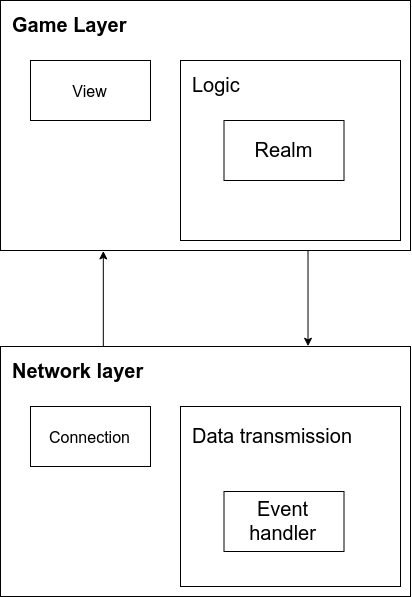
\includegraphics[scale=0.4]{GameBank}
 \caption{GameBank architecture}
 \label{fig:gbArchitecture}
\end{figure}

The game layer simply takes the events coming from the network transmissions, 
and it stores the data in a Realm database\footnote{\url{https://realm.io/}} 
through the logic layer, that is based on events too. Finally, the views, that 
are what the user sees and interact with, subscribe to events coming from logic 
and bluetooth parts, allowing them to be updated by the \textit{on change 
callbacks}.

\subsection{Game creation}

In the section above we briefly talked how a match is created: here we are 
going to describe in the details the procedure we have designed to connect the 
Bluetooth devices and to start a match.

When a user opens a match, in the network layer a Bluetooth socket is opened 
and set up for an incoming connection. When a client connects to the host, to 
host, first it saves its UUID, its username and its profile picture into a 
\texttt{BTBundle} (a rendezvous) and then it sends it back.
This is the slower phase of the connection: indeed transferring the profile 
picture is a heavy task for Bluetooth, that takes seconds to transfer the image, 
even if we used compression techniques to reduce images dimensions. We called 
this event \texttt{MEMBER\_CONNECTED}. Since the connection of a new member 
needs to be broadcasted to everyone, the host forwards to all the other clients 
already in the lobby the \texttt{BTBundle} the new member initially sent, acting 
in a transparent way. When this phase is completed, the host informs the new 
client with all the informations regarding the match, as the lobby name and a 
list of players already connected. We labelled this event as 
\texttt{CURRENT\_STATE}. In case the match comes from a previous save, the new 
client receives, in the same event, all the transactions performed before.

\begin{figure}[t]
 \centering
 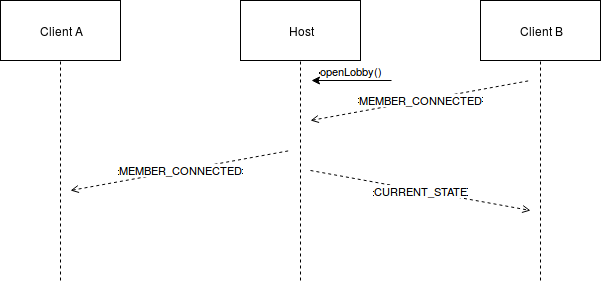
\includegraphics[scale=0.42]{ConnectionSchema}
 \caption{Schema of client-host connection}
 \label{fig:gbConnectionSchema}
\end{figure}

A match can start when all the members are ready. In order to do so, users have 
to check the option in the lobby. When this action is performed, a 
\texttt{MEMBER\_READY} event is triggered. This event is broadcasted to everyone 
to allow the other clients to update their UI.

When the host choose to start the match, the event \texttt{START} is 
broadcasted too, making the clients start the dashboard activity.

\begin{figure}[t]
 \centering
 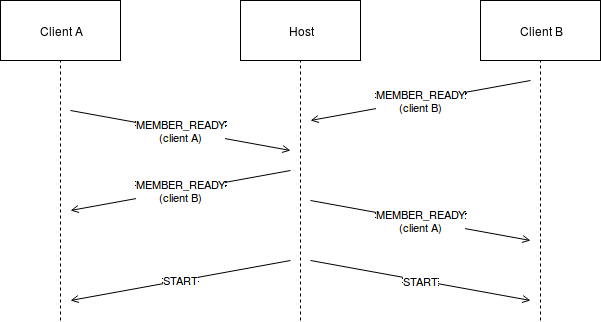
\includegraphics[scale=0.42]{StartMatch}
 \caption{Schema of a start of a match}
 \label{fig:gbStartMatch}
\end{figure}

\subsection{Data transmission}

We decided to transfer all the data in JSON format, encoding with base64 all the
non-text content.
Of all the transport protocols available in Bluetooth, we have chosen RFCOMM to 
carry data between devices. First of all, RFCOMM has a behaviour similar to TCP 
and it is recommend for data transfers~\cite{bisdikian01}. Secondly, Android 
offers a Bluetooth API based on RFCOMM that gives the possibility to open 
sockets and treat them as standard TCP connections.
RFCOMM is usually referred as a serial port emulator, it is make on top of 
the L2CAP protocol~\cite{bisdikian01}, and allows up to 60 simultaneous 
connections between two Bluetooth devices~\cite{aneesh12}.

The communications during the game creation are synchronous when 
\texttt{MEMBER\_CONNECTED} and \texttt{CURRENT\_STATE} events happen, while 
they are asynchronous for packets regarding \texttt{POKE} 
and \texttt{MEMBER\_READY} actions. Instead, during the match, all the 
communications are performed synchronously since the order of the transactions 
is very important.

\subsection{Known issues}

During the app development we have faced some issues that we were able to 
partially solve.

\subsubsection{Image dimensions}

As already said, images too large cause long transmission times with bluetooth, 
an since we transfer data  in the main thread, this results in the application 
hanging while transferring it, providing bad usability. In order to partially 
solve this problem, we have reduced images dimension, scaling them to a default 
one, converting them to the JPEG format and reducing their overall quality. A 
definitive solution would be using a thread different from the one running the 
user interface, displaying to the user a loading message during bluetooth 
transmissions.

\subsubsection{S3 first application run}

We found that using the Samsung S3 (I9300) model permissions were not granted 
correctly, consequently we were not able to save the user's photos properly and 
thus to send her profile picture at the first application run. Debugging did 
not produce any evidence of bugs in our application, since the permissions 
were granted during the start up time.
We address this issue to the custom ROM installed on the smartphone, LineageOS 
(Android Nougat 7.1), which probably has some problem to handle authorizations 
only on S3 smartphones. In fact, we tried this ROM on a Nexus 5 and we have not 
noticed any erroneous behaviour. To confirm our guesses, we tried other 
applications available on the Google's Play Store, experiencing the same 
problem.

\subsubsection{Realm database}

Realm, the database GameBank uses to store data, generated some problem 
especially regarding extrapolating data from it. In fact, Realm create 
particular istances of classes that act as proxy from the real data contained 
in the database, to save RAM memory. This made difficult to send these objects 
via Bluetooth. Initially we tried to send/receive them with 
\texttt{ObjectOutputStream} and \texttt{ObjectInputStream}, but we discovered 
that Realm objects were not serializable. Then, we tried to convert them into 
JSON objects, but even here we faced some problems because we had to manually 
implement serializer/deserializer handlers for the \texttt{Gson} framework we 
used to manipulate JSONs, since these Realm proxies didn't provide 
automatically data at conversion time.

On top of that, the framework revealed to be very difficult to decuple with the 
rest of the application, resulting sometimes in a blending between the view and 
the logic modules.
